\documentclass[12pt,a4paper,oneside]{report}

% ==========================================
% PACKAGES
% ==========================================
\usepackage{geometry}
\geometry{a4paper, left=1.2in, right=1in, top=1in, bottom=1in}
\usepackage[utf8]{inputenc}
\usepackage[T1]{fontenc}
\usepackage{graphicx}
\usepackage{hyperref}
\usepackage{fancyhdr}
\usepackage{titlesec}
\titleformat{\chapter}[display]
  {\normalfont\huge\bfseries}{\chaptertitlename\ \thechapter}{10pt}{\Huge}
\titlespacing*{\chapter}{0pt}{-40pt}{30pt} % Reduces massive top margin before chapters
\usepackage{booktabs}
\usepackage{enumitem}
\usepackage{longtable}
\usepackage{mdframed}
\usepackage{tabularx}
\usepackage{xcolor}
\usepackage{setspace}
\usepackage{float}
\usepackage{listings}
\usepackage{caption}

% ==========================================
% TIKZ PACKAGE & LIBRARIES (FOR ARCHITECTURE DIAGRAMS)
% ==========================================
\usepackage{tikz}
\usetikzlibrary{shapes.geometric, arrows, positioning, fit, calc, backgrounds}

% Tikz styles setup for flowcharts and diagrams
\tikzstyle{process} = [rectangle, minimum width=3cm, minimum height=1cm, text centered, draw=black, fill=blue!10, rounded corners]
\tikzstyle{database} = [cylinder, shape border rotate=90, aspect=0.25, draw=black, fill=purple!10, minimum height=1.5cm, minimum width=2.5cm, text centered]
\tikzstyle{cloudnode} = [ellipse, draw=black, fill=green!10, minimum height=1cm, minimum width=2.5cm, text centered]
\tikzstyle{arrow} = [thick,->,>=stealth]

% ==========================================
% CUSTOM COLORS & HYPERLINKS
% ==========================================
\definecolor{primary}{RGB}{0, 83, 156}
\definecolor{codebg}{rgb}{0.95,0.95,0.95}

\hypersetup{
    colorlinks=true,
    linkcolor=primary,
    filecolor=magenta,      
    urlcolor=blue,
    pdftitle={Get Hired (JobSeg Portal) - SRS and Technical Report},
}

% ==========================================
% CODE SNIPPETS STYLING
% ==========================================
\lstset{
    backgroundcolor=\color{codebg},   
    basicstyle=\ttfamily\footnotesize,
    breaklines=true,                 
    captionpos=b,                    
    keepspaces=true,                 
    numbers=left,                    
    numbersep=5pt,                  
    showspaces=false,                
    showstringspaces=false,
    showtabs=false,                  
    tabsize=2
}

% ==========================================
% HEADER & FOOTER
% ==========================================
\pagestyle{fancy}
\fancyhf{}
\fancyhead[L]{\textsl{Get Hired - System Documentation}}
\fancyfoot[C]{\textbf{\thepage}}
\renewcommand{\headrulewidth}{0.4pt}
\renewcommand{\footrulewidth}{0.4pt}
\setlength{\headheight}{15pt}

\begin{document}

\setstretch{1.3} % 1.3 line spacing for professional readability

% ==========================================
% TITLE PAGE
% ==========================================
\begin{titlepage}
    \begin{center}
        \vspace*{2cm}
        
        {\Huge \textbf{GET HIRED}} \\
        \vspace{0.3cm}
        {\Large \textit{(The JobSeg Portal)}}
        
        \vspace{1.5cm}
        {\Large \textbf{SOFTWARE REQUIREMENTS SPECIFICATION}} \\
        \vspace{0.2cm}
        {\normalsize \textbf{\& COMPREHENSIVE TECHNICAL ARCHITECTURE REPORT}}
        
        \vspace{2cm}
        
        \textbf{Developed for:} \\
        \vspace{0.2cm}
        India's Emerging Engineers \& Professionals
        
        \vspace{1.5cm}
        
        {\large \textbf{Supervised By:}} \\
        \vspace{0.1cm}
        {\large \textbf{[Insert Faculty Name]}} \\
        \textit{[Insert Faculty Designation]} \\
        
        \vspace{1.5cm}
        
        {\large \textbf{Prepared By:}} \\
        \vspace{0.5cm}
        
        \begin{minipage}[t]{0.33\textwidth}
            \begin{center}
                \textbf{[Member 1 Name]} \\
                Regd. No: [ID 1]
            \end{center}
        \end{minipage}%
        \begin{minipage}[t]{0.33\textwidth}
            \begin{center}
                \textbf{[Member 2 Name]} \\
                Regd. No: [ID 2]
            \end{center}
        \end{minipage}%
        \begin{minipage}[t]{0.33\textwidth}
            \begin{center}
                \textbf{[Member 3 Name]} \\
                Regd. No: [ID 3]
            \end{center}
        \end{minipage}
        
        \vfill
        
        \rule{0.8\textwidth}{0.4pt} \\
        \vspace{0.5cm}
        {\large \textbf{Date:} \today} \\
        {\large \textbf{Version:} 1.0.0}
        
    \end{center}
\end{titlepage}

% ==========================================
% DECLARATION & ACKNOWLEDGEMENT
% ==========================================
\chapter*{Declaration}
\addcontentsline{toc}{chapter}{Declaration}
We hereby declare that the software architecture, design, and internal specifications documented in this report for the project titled \textbf{"Get Hired (JobSeg Portal)"} represent original developmental tracking and system analysis. The documentation comprehensively mirrors the active MERN stack codebase, its underlying databases, and third-party integrations as of the compilation date.

\vspace{1cm}

\chapter*{Abstract}
\addcontentsline{toc}{chapter}{Abstract}
The \textbf{Get Hired} platform represents a paradigm shift in how employment opportunities are curated and delivered to candidates, particularly within the Indian technological sector. Traditional job boards require deliberate manual intervention from companies to post openings. In contrast, this project engineers a completely autonomous \textbf{Job Aggregation Module} capable of scraping, standardizing, and deduplicating job data from over six recognized global APIs (including Adzuna, JSearch, Remotive, and The Muse). 

Beyond aggregation, the platform incorporates advanced \textbf{Generative AI models} (such as Google Gemini and Meta LLaMA-3) to act as an Applicant Tracking System (ATS) proxy and an AI Career Coach, evaluating user resumes against real-time listings to yield a quantifiable compatibility metric. The architecture resolves heavy workloads securely via Node.js cron scheduling, caching, JWT-based security layers, and `$text$' indexing within MongoDB. This report formalizes the operational behaviors, entity relationships, security implementations, and system protocols required to maintain the platform's lifecycle.

\newpage

% ==========================================
% TABLE OF CONTENTS & LISTS
% ==========================================
\pagenumbering{roman}
\tableofcontents
\newpage
\listoftables
\newpage
\listoffigures
\newpage
\pagenumbering{arabic}

% ==========================================
% CHAPTER 1: INTRODUCTION
% ==========================================
\chapter{Introduction}

\section{1.1 Project Purpose}
The purpose of \textbf{Get Hired} is to streamline the career progression of software developers and general job seekers. It aims to eliminate the friction of searching across fragmented job boards by automatically consolidating openings into one standardized environment, augmented by robust AI-driven profile analytics. 

\section{1.2 Scope of the Document}
This System Requirements Specification (SRS) covers the architectural design, database schematics, core functional constraints, application workflows, and application programming interface (API) definitions. It is intended for software engineers, database administrators, and prospective maintainers scaling the project.

\section{1.3 Target Audience}
\begin{itemize}
    \item \textbf{Candidates (End-Users):} Freshers, juniors, and senior-level staff seeking employment.
    \item \textbf{System Administrators:} Quality assurance managers monitoring scraper health, resolving false entries, or tweaking scheduler chronologies.
\end{itemize}

\section{1.4 Existing Systems and Drawbacks}
Existing systems such as LinkedIn, Naukri, or Indeed largely operate on a push-model—requiring recruiters to push job details onto the platform. 
Drawbacks include:
\begin{itemize}
    \item Candidate profiles are seldom matched contextually against job descriptions using generative parsing.
    \item Remote jobs and niche openings on external company domains often slip through standard keyword searches.
    \item Standard ATS filters reject candidates invisibly. 
\end{itemize}
Our proposed system solves this using \textit{passive ingestion} (pulling data periodically) and providing transparent ATS score analytics back to the candidate.

% ==========================================
% CHAPTER 2: SYSTEM ARCHITECTURE
% ==========================================
\chapter{System Architecture}

\section{2.1 High-Level Architecture}
The system executes upon the modernized \textbf{MERN Stack}.

\subsection{Frontend Environment}
The client is established using \textbf{React.js} (React 19+) running atop the \textbf{Vite} bundler for High-Speed Module Replacement (HMR). 
\begin{itemize}
    \item \textbf{State Contexts:} Global environments control \texttt{AuthContext} and \texttt{ThemeContext}.
    \item \textbf{Routing:} Client-side URL resolution is mapped by \texttt{React Router}.
    \item \textbf{Styling Protocol:} The platform strictly utilizes massive vanilla CSS architectures prioritizing Glassmorphism aesthetics without the bloat of frameworks like Tailwind, guaranteeing uniquely tailored interactive metrics.
\end{itemize}

\subsection{Backend Environment}
The server layer communicates exclusively via REST protocols via \textbf{Node.js} and \textbf{Express.js}.
\begin{itemize}
    \item \textbf{Concurrency Regulation:} Integrates libraries like \texttt{p-limit} to prevent API throttling during aggressive scraper loops.
    \item \textbf{Routine Automation:} Employs \texttt{node-cron} enforcing chron-job actions (aggregations firing every 6 hours, dead-job cleanup daily at 2:00 AM IST).
\end{itemize}

\subsection{Database Topology}
Data permanence relies on \textbf{MongoDB}. Interfacing occurs through Mongoose Object Data Modeling (ODM). Heavy usage of \texttt{\$text} indexing strategies allows multi-millisecond query answers for robust text filtering over millions of characters.

\vspace{0.5cm}
\begin{figure}[H]
    \centering
    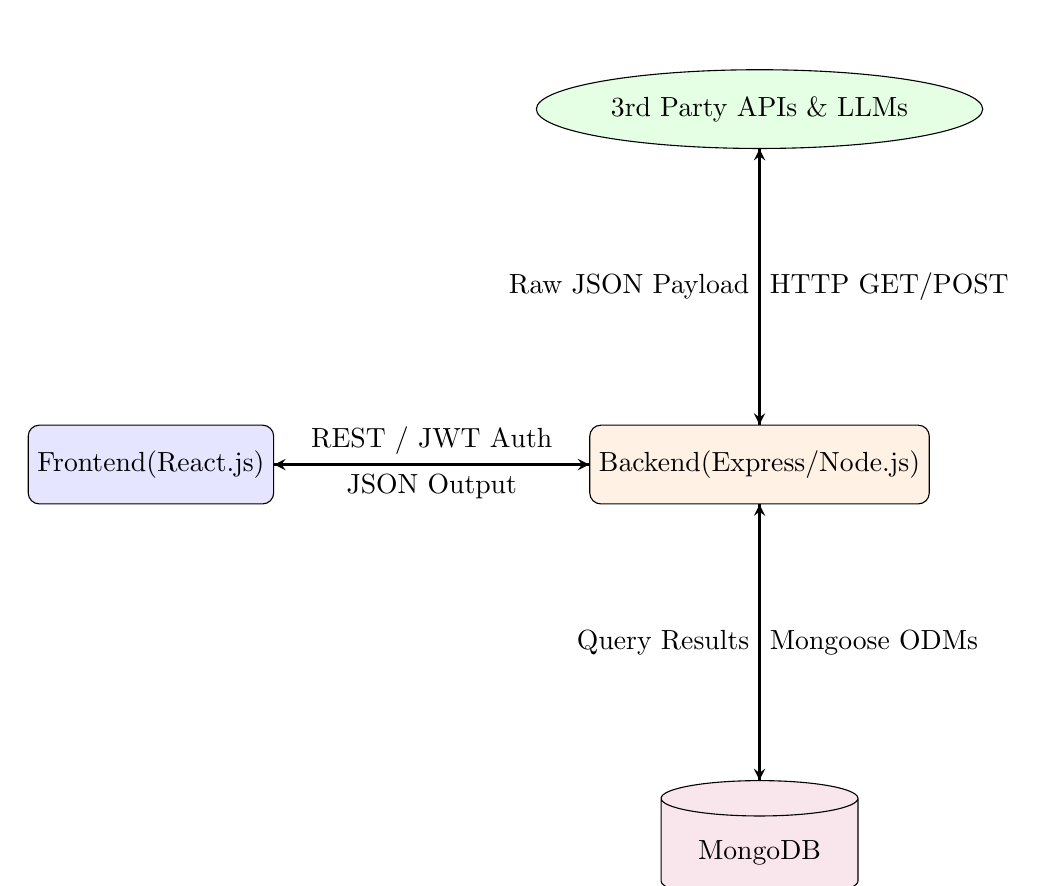
\begin{tikzpicture}[node distance=2.5cm]
        \node (client) [process, fill=blue!10] {Frontend \newline (React.js)};
        \node (server) [process, fill=orange!10, right=of client, xshift=1.5cm] {Backend \newline (Express/Node.js)};
        \node (db) [database, below=of server, yshift=-1cm] {MongoDB};
        \node (apis) [cloudnode, above=of server, yshift=1cm] {3rd Party APIs \& LLMs};
        
        \draw [arrow] (client) -- node[anchor=south] {REST / JWT Auth} (server);
        \draw [arrow] (server) -- node[anchor=north] {JSON Output} (client);
        
        \draw [arrow] (server) -- node[anchor=west] {Mongoose ODMs} (db);
        \draw [arrow] (db) -- node[anchor=east] {Query Results} (server);
        
        \draw [arrow] (server) -- node[anchor=west] {HTTP GET/POST} (apis);
        \draw [arrow] (apis) -- node[anchor=east] {Raw JSON Payload} (server);
    \end{tikzpicture}
    \caption{High-Level MERN Stack Application Architecture}
    \label{fig:highlevel_arch}
\end{figure}

\section{2.2 The Aggregation \& Workflow Pipeline}
\textbf{The Workflow consists of four distinct phases:}
\begin{enumerate}
    \item \textbf{Acquisition:} The \texttt{JobAggregator} instantiates API connections pushing headers matching RapidAPI configurations to Adzuna or JSearch endpoints.
    \item \textbf{Formatting:} The JSON responses are fundamentally chaotic. The backend mapping classes sanitize fields (Extracting `30k-40k INR' into rigid min/max integer objects).
    \item \textbf{Deduplication (Hashing Vector):}
    A cryptographic fingerprint algorithm combines \texttt{lowercase("Title" + "Company" + "City")}. If the MongoDB \texttt{fingerprint} string registers a collision during a batch insertion, the record is flagged and skipped cleanly.
    \item \textbf{Presentation:} Once settled into the collection, data is immediately reachable over port 5001 APIs and injected into the frontend DOM elements dynamically.
\end{enumerate}

\vspace{0.5cm}
\begin{figure}[H]
    \centering
    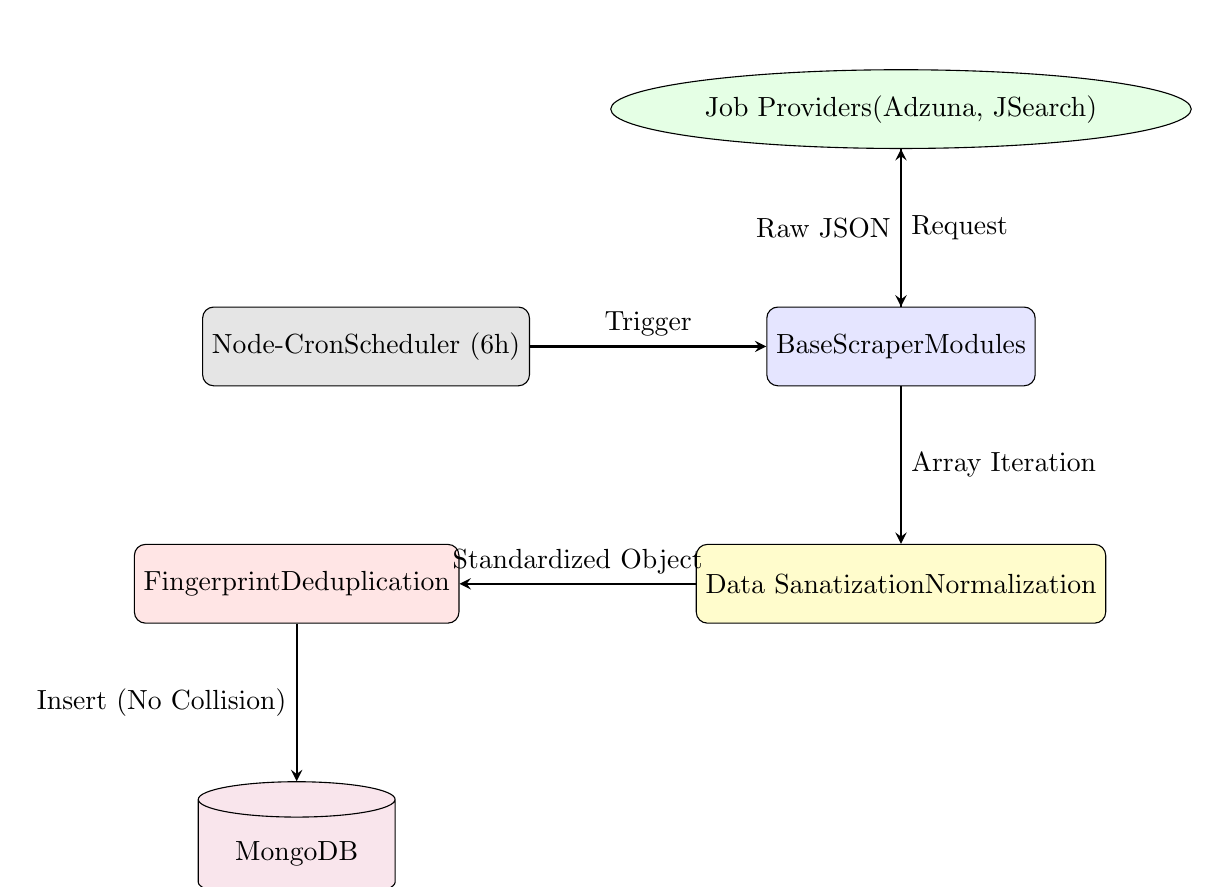
\begin{tikzpicture}[node distance=1.5cm]
        \node (cron) [process, fill=gray!20] {Node-Cron \newline Scheduler (6h)};
        \node (scrapers) [process, fill=blue!10, right=of cron, xshift=1.5cm] {BaseScraper \newline Modules};
        \node (sources) [cloudnode, above=of scrapers, yshift=0.5cm] {Job Providers \newline (Adzuna, JSearch)};
        \node (norm) [process, fill=yellow!20, below=of scrapers, yshift=-0.5cm] {Data Sanatization \newline Normalization};
        \node (dedup) [process, fill=red!10, left=of norm, xshift=-1.5cm] {Fingerprint \newline Deduplication};
        \node (db) [database, below=of dedup, yshift=-0.5cm] {MongoDB};
        
        \draw [arrow] (cron) -- node[anchor=south] {Trigger} (scrapers);
        \draw [arrow] (scrapers) -- node[anchor=west] {Request} (sources);
        \draw [arrow] (sources) -- node[anchor=east] {Raw JSON} (scrapers);
        
        \draw [arrow] (scrapers) -- node[anchor=west] {Array Iteration} (norm);
        \draw [arrow] (norm) -- node[anchor=south] {Standardized Object} (dedup);
        \draw [arrow] (dedup) -- node[anchor=east] {Insert (No Collision)} (db);
    \end{tikzpicture}
    \caption{Job Aggregator \& Deduplication Data Flow}
    \label{fig:aggregator_pipeline}
\end{figure}

% ==========================================
% CHAPTER 3: REQUIREMENT SPECIFICATIONS
% ==========================================
\chapter{Requirement Specifications}

\section{3.1 Hardware and Software Constraints}
\textbf{Minimum Server Resources:}
\begin{itemize}
    \item Architecture: 64-bit OS (Linux/Unix preferred)
    \item Memory: 4 GB RAM (To handle parsing buffers for heavy PDF loads)
    \item Storage: 20 GB SSD (Log retention \& indexing constraints)
\end{itemize}
\textbf{Software Dependencies:} Node.js v24+, MongoDB v6.0+, and an external PDF processor/LLM API hook.

\section{3.2 Functional Requirements (FR)}

\subsection{FR-1: Automated Scraper Operations}
The system MUST dynamically fetch data without user input. Administrators MUST have access to manually override endpoints to force a re-synchronization per respective channel.

\subsection{FR-2: AI System Tolerance}
The AI mechanism MUST perform heuristic fallbacks. Should Google Gemini limits exhaust, or network timeouts trigger, local NLP (Natural Language Processing) regex parameters MUST parse basic text logic to maintain platform stability.

\subsection{FR-3: User Profiles and Activity}
Candidates MUST be able to apply explicit toggles protecting UI feeds (e.g., toggling ``International Jobs'' off filters only India/Remote focused arrays).

\section{3.3 Non-Functional Requirements (NFR)}

\subsection{NFR-1: System Security}
Traffic directed toward \texttt{/api/admin/*} heavily limits IPs to 1000 requests per 15-minute window utilizing \texttt{express-rate-limit}. Environment keys and Secrets MUST remain encrypted locally in \texttt{.env}.

\subsection{NFR-2: Time to Live (TTL) Protocols}
Database hygiene dictates that \texttt{SyncLogs} generated by scraping engines MUST self-destruct utilizing MongoDB TTL properties after 30 days to prevent cluster degradation. Jobs older than 60 days MUST automatically update to \texttt{isActive: false}.

% ==========================================
% CHAPTER 4: CORE MODULES & FEATURES
% ==========================================
\chapter{Detailed Functional Modules}

\section{4.1 Aggregation Scraper Engines}
Built under a unified interface class termed \texttt{BaseScraper}, the system adapts various inputs:
\begin{itemize}
    \item \textbf{Adzuna \& JSearch:} Require strict API authentication keys parsed from the environment layer. Offers complex parameters tracking Indian salary scales (LPA/Crores).
    \item \textbf{RemoteOK, Remotive, Arbeitnow, The Muse:} Free APIs accessed via axios fetching strings. Extracted parameters require heavier Regex extraction to pull location semantics.
\end{itemize}
India detection logic validates string intersections mapping over 100 Indian state and city titles, enforcing localization.

\section{4.2 AI Resume Parser \& ATS Grader}
Traditional ATS evaluates strict 1-to-1 keyword overlaps. Modifying this logic:
The system parses candidate PDF buffers into raw strings. The data is transferred via streaming requests to the LLM (Gemini 1.5 Flash). A strict prompt asks the LLM to output a precise JSON schema responding with:
\begin{lstlisting}[language=json, caption=LLM Desired Return Entity]
{
  "score": 85,
  "matched_skills": ["React", "Express", "MongoDB"],
  "missing_keywords": ["Kubernetes", "AWS EC2"]
}
\end{lstlisting}

\vspace{0.5cm}
\begin{figure}[H]
    \centering
    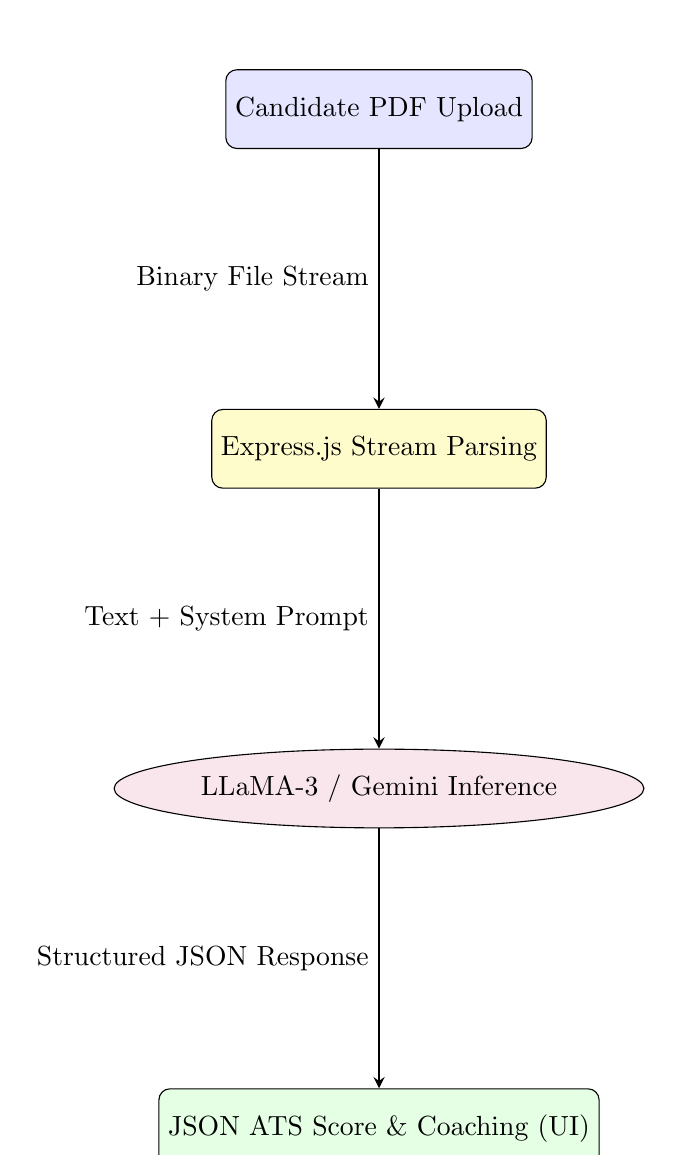
\begin{tikzpicture}[node distance=2.5cm]
        \node (user) [process] {Candidate PDF Upload};
        \node (buffer) [process, fill=yellow!20, below=of user, yshift=-0.8cm] {Express.js Stream Parsing};
        \node (llm) [cloudnode, fill=purple!10, below=of buffer, yshift=-0.8cm] {LLaMA-3 / Gemini Inference};
        \node (response) [process, fill=green!10, below=of llm, yshift=-0.8cm] {JSON ATS Score \& Coaching (UI)};
        
        \draw [arrow] (user) -- node[anchor=east] {Binary File Stream} (buffer);
        \draw [arrow] (buffer) -- node[anchor=east] {Text + System Prompt} (llm);
        \draw [arrow] (llm) -- node[anchor=east] {Structured JSON Response} (response);
    \end{tikzpicture}
    \caption{AI Applicant Tracking System (ATS) Parser Architecture}
    \label{fig:ai_parser}
\end{figure}

\section{4.3 Administrator Control Base}
By logging in through standard channels, individuals holding an \texttt{admin} role trigger layout shifts rendering the \textbf{Admin Interface}.
Visualizations (Area/Pie Charts) evaluate metrics over the last 30 intervals. Bulk actions allow administrators to transmit arrays of \texttt{Job IDs} deleting hundreds of failed job parsing attempts instantaneously.

% ==========================================
% CHAPTER 5: DATABASE SCHEMAS
% ==========================================
\chapter{System Database Design}
The relational boundaries mapped in MongoDB NoSQL format guarantee low latency mapping.

\section{5.1 Primary Models}

\subsection{User Schematic}
Manages identity access and profile details.
\begin{itemize}
    \item \textbf{email:} Unique index string.
    \item \textbf{password:} String array secured through \texttt{Bcrypt.js} hashing (12 rounds). Explicitly disabled in default queries (\texttt{select: false}).
    \item \textbf{preferences:} Holds arrays mapping desired \textit{Locations, JobTypes, ExperienceLevels}.
\end{itemize}

\subsection{Job Schematic}
Registers the standardized payload extracted globally.
\begin{itemize}
    \item \textbf{company:} Nested payload ensuring \texttt{\{name, logo, verified\}} flags.
    \item \textbf{fingerprint:} Crucial deterministic hash ensuring identical occurrences across JSearch and Adzuna do not duplicate interface listings.
    \item \textbf{isInternational:} Boolean triggered if scraping engines notice the geographical center is outside the subcontinent \textit{AND} the job is not explicit to Remote culture.
\end{itemize}

\subsection{Source Schematic \& SyncLogs}
Metadata collections analyzing system wellness.
\begin{itemize}
    \item \textbf{rateLimit:} Contains \texttt{maxRequests} validating safe query volumes protecting backend IP bans.
    \item \textbf{SyncLog:} Exposes \texttt{\{jobsFetched, jobsDuplicate, errors[]\}} for granular administrative analysis post-cron loop execution.
\end{itemize}

% ==========================================
% CHAPTER 6: API REFERENCE (REST)
% ==========================================
\chapter{Application Programming Interfaces (REST Network)}

\section{6.1 Routing and Endpoints}
Below defines the principal backend interfaces exposed on Port 5001.

\begin{table}[H]
\centering
\caption{Public Facing Endpoints}
\renewcommand{\arraystretch}{1.5}
\begin{tabularx}{\textwidth}{|l|l|c|X|}
\hline
\textbf{Method} & \textbf{Endpoint} & \textbf{Security} & \textbf{Purpose} \\ 
\hline
GET & \texttt{/api/jobs} & None & Fetches active aggregations. \\
\hline
GET & \texttt{/api/jobs/search} & None & Executes complex \$regex \& \$text arrays resolving job parameters. \\
\hline
GET & \texttt{/api/jobs/skills} & None & Analyzes active arrays generating a hash map of trending industry elements.\\
\hline
\end{tabularx}
\end{table}

\begin{table}[H]
\centering
\caption{Protected Auth and Application Endpoints}
\renewcommand{\arraystretch}{1.5}
\begin{tabularx}{\textwidth}{|l|l|c|X|}
\hline
\textbf{Method} & \textbf{Endpoint} & \textbf{Security} & \textbf{Purpose} \\ 
\hline
POST & \texttt{/api/auth/register} & None & Enacts bcrypt rounds and generates User class. \\
\hline
POST & \texttt{/api/applications} & JWT Req & Initiates relationship link validating User ObjectId against Job ObjectId.\\
\hline
PUT & \texttt{/api/applications/:id} & JWT Req & Re-renders the status enum spanning `interviewing' vs `rejected'.\\
\hline
\end{tabularx}
\end{table}

\begin{table}[H]
\centering
\caption{Administrative Command Routes}
\renewcommand{\arraystretch}{1.5}
\begin{tabularx}{\textwidth}{|l|l|c|X|}
\hline
\textbf{Method} & \textbf{Endpoint} & \textbf{Security} & \textbf{Purpose} \\ 
\hline
POST & \texttt{/api/admin/jobs/sync/:id} & Admin & Bypasses cron timeline instantiating immediate HTTP scrape pipelines against explicit targets.\\
\hline
DELETE & \texttt{/api/admin/jobs/expired} & Admin & Mass cleanses nodes past TTL or manual expiration properties.\\
\hline
PUT & \texttt{/api/admin/users/:id/role} & Admin & Mutates normal user access, granting admin clearances.\\
\hline
\end{tabularx}
\end{table}

% ==========================================
% CHAPTER 7: SECURITY \& LIMITATIONS
% ==========================================
\chapter{Security Mechanisms and Known Limitations}

\section{7.1 Implemented Defenses}
\textbf{Cross-Site Scripting (XSS) \& Injection Protection:} Parameter sanitization occurs actively through \texttt{Joi} validation arrays checking standard `\texttt{req.body}` payloads prior to database insertions. \\
\textbf{Password Hiding:} At no phase does the `\texttt{/me}` controller transmit password parameters due strictly to the Mongoose \texttt{select: false} modifier configuration.

\section{7.2 Existing Analytical Vulnerabilities (Flaws)}
During detailed peer-review architecture evaluations, a few missing necessities became apparent. The future scope must aggressively address:
\begin{itemize}
    \item \textbf{Backend Administration Protection Gap:} The frontend aggressively blocks standard consumers from reaching `/admin` interfaces by parsing the state Context's \texttt{user.role} verification. Unfortunately, the REST backend controller for \texttt{api/admin/*} is currently lacking sequential enforcement of \texttt{authRequired} and \texttt{adminRequired} middleware chains. This subjects sensitive API endpoints strictly to rate-limiting protocol dependency, opening vectors to potential rogue manual HTTP sweeps.
    \item \textbf{Incomplete File Upload Logic:} While Candidate Application arrays harbor strings for a \texttt{resumeUrl}, physical blob storage algorithms integrating AWS S3 architecture or distinct Multer streams are pending.
    \item \textbf{User Verification Tunnels:} The JWT creation happens instantaneously. Strict transactional email confirmation sequences linking NodeMailer / SendGrid templates are presently skipped.
\end{itemize}

% ==========================================
% CHAPTER 8: CONCLUSIONS
% ==========================================
\chapter{Conclusion}
The **Get Hired (JobSeg Portal)** introduces a high-performing backend logic circuit dedicated natively towards career navigation. Through intricate scheduled Node.js cycles manipulating vast text-indexes stored in MongoDB, users are granted transparent insights into ATS frameworks while avoiding redundant duplicates previously polluting Indian markets. System deployment readies developers for complex expansions regarding generative career mapping integrations.

\end{document}
